\documentclass{wfiisul}
%

\usepackage[utf8]{inputenc}
\usepackage{amsmath}
\usepackage{tabularx}
\usepackage[hidelinks]{hyperref}
\usepackage{afterpage}

%\usepackage{pdflscape}
%\usepackage{afterpage}
%\usepackage{changepage}
%\usepackage{caption}
%\usepackage{rotating} %for sidewisetable
%\usepackage{makecell}
%\usepackage{boldline}
%\usepackage{amsthm}
%\usepackage{amsopn}
% włączenie polskich znaków
%\usepackage{lmodern}
%\usepackage{wrapfig}
%\usepackage[table]{xcolor}

\usepackage{framed}
\usepackage{listings}
\usepackage[most]{tcolorbox}



\begin{document}

\tytul{Tytuł Pracy Dyplomowej }

\autor{Imie Nazwisko}
\nralbumu{****}

\promotor{***}
\katedra{****}

\kierunek{informatyka}
%\kierunek{fizyka}

%% JEŚLI INFORMATYKA
\specjalnosc{informatyka stosowana}
%% DLA PRAC INŻYNIERSKICH
\typpracy{inżynierska}
\specjalizacja{****}

%% DLA PRAC MAGISTERSKICH
%\typpracy{magisterska}
%\sciezka{***}

%% JEŚLI FIZYKA
%% DLA PRAC LICENCJACKICH
%\typpracy{licencjacka}
%\sciezka{***}

%% DLA PRAC MAGISTERSKICH
%\typpracy{magisterska}
%\sciezka{***}



\stronatytulowa


\chapter{Wykorzystanie stylu w pracy dyplomowej}

Poniższy dokument jest przykładowym zastosowaniem szablonu .cls pracy dyplomowej na Wydziale Fizyki i Informatyki Stosowanej UŁ. Każdy rozdział pracy może dzielić się na sekcje i pod-sekcje. Spis treści budowany jest z wykorzystaniem elementów : {\textbackslash}chapter, {\textbackslash}section i {\textbackslash}subsection. Szablon zakłada wydruk dwustronicowy, z tego powodu każdy nowy rozdział rozpoczyna się na stronie nieparzystej.

Praca musi być przygotowana zgodnie z Procedurą dyplomowania przyjętą na Wydziale Fizyki i Informatyki Stosowaniej Uniwersytetu Łódzkiego \cite{Procedura_dyplomowania}.
\section{System \LaTeX}
Można znaleźć wiele źródeł na temat systemu \LaTeX \cite{latex_wiki}.

\section{Wykorzystanie stylu pracy dyplomowej}
Zasady wykorzystania stylu wfisul.cls, na początku pliku należy wykorzystać klasę wfiisul, plik cls musi być dostępny w trakcie kompilacji. Źródła .tex niniejszego dokumentu zawierają wszystkie niezbędne elementy dla prac inżynierskich z informatyki, elementy dla innych typów prac zostały zakomentowane, w celu wykorzystanie wystarczy odpowiednia modyfikacja źródła pliku. 

\begin{lstlisting}[language=TeX, basicstyle=\ttfamily]
\documentclass{wfiisul}
\end{lstlisting}

Na początku dokumentu należy zdefiniować wszystkie predefiniowane parametry pracy, nie zapominając odpowiednim  uzupełnieniu danych jak tytuł pracy, imie nazwisko autora, nr albumu itp.. Należy pamiętać o elementach związanych z kierunkiem czy typem pracy.

\begin{lstlisting}[language=TeX, basicstyle=\ttfamily, , mathescape=true]
\begin{document}
\tytul{Tytu$\text{ł}$ pracy dyplomowej}
\autor{Imie Nazwisko}
\nralbumu{****}
\promotor{***}
\katedra{****}
\end{lstlisting}

Następnie zdefiniować elementy odpowiednie dla kierunku i typu pracy dyplomowej

\subsection{Kierunek fizyka}

\subsubsection{Praca licencjacka}
\begin{lstlisting}[language=TeX, basicstyle=\ttfamily]
\kierunek{fizyka}
\typpracy{licencjacka}
\sciezka{***}
\end{lstlisting}

\subsubsection{Praca magisterska}
\begin{lstlisting}[language=TeX, basicstyle=\ttfamily]
\kierunek{fizyka}
\typpracy{magisterska}
\sciezka{***}
\end{lstlisting}

\subsection{Kierunek informatyka}
\subsubsection{Praca inżynierska}
\begin{lstlisting}[language=TeX, basicstyle=\ttfamily, mathescape=true]
\kierunek{informatyka}
\specjalnosc{informatyka stosowana}
\typpracy{in$\text{ż}$ynierska}
\specjalizacja{****}
\end{lstlisting}

\subsubsection{Praca magisterska}
\begin{lstlisting}[language=TeX, basicstyle=\ttfamily]
\kierunek{informatyka}
\specjalnosc{informatyka stosowana}
\typpracy{magisterska}
\sciezka{****}
\end{lstlisting}

\subsection{Utworzenie strony tytułowej}

Po wypełnieniu wszystkich niezbędnych parametrów pracy należy wydać instrukcję  dodania strony tytułowej:

\begin{lstlisting}[language=TeX, basicstyle=\ttfamily, inputencoding=utf8, extendedchars=false]
\stronatytulowa
\end{lstlisting}


\chapter{Język pracy}

\section{Spacje i znaki interpunkcyjne}
System latex sam radzi sobie ze wielokrotnymi spacjami, jednakże nie należy ich stosować w tekście. Nowy akapit oznacza się jedną pustą linią w dokumencie .tex. 

Znaki interpunkcyjne takie jak przecinek (,), kropka (.), dwukropek (:), średnik (;), znak zapytania (?), wykrzyknik (!), zamknięcie dowolnego nawiasu (]\})>), zamknięcie cudzysłowu ('' lub ') nie mogą być nigdy poprzedzone spacją. Bezpośrednio po wymienionych znakach może wystąpić wyłącznie spacja, znak nowego akapitu lub inny znak interpunkcyjny. Po znakach otwierających dowolnego nawiasu ([\{(<) lub otwarcia cudzysłowu (`` lub `) nigdy nie należy używać spacji. Spację używamy przed tymi znakami. Nie należy rozpoczynać akapitu od spacji – przerwa ta jest dodawana  automatycznie przez system latex.

Dodatkowo sugeruje się stosowanie twardych spacji w celu unikania wszelkiego rodzaju sierotek, przed ostatecznym wysłaniem pracy do APD należy sprawdzić czy nie występują  bękarty, sierotki, wdowy i szewcy \cite{Bekart}.

\section{Wzory matematyczne}
W systemie latex występują dwa główne rodzaje wzorów, wstawiane w element zdania $E = mc^2$, tworzone za pomocą środowiska \$\dots\$, jak i umieszczane w osobnych linijkach z wykorzystaniem środowisk: \textit{equation, equation* (\textbackslash[\dots\textbackslash])}
\begin{equation}\label{eq:wn}
W(n) = \bigotimes_{n} W(1),
\end{equation}
where:
\begin{equation}\label{eq:w1}
W(1) = \begin{bmatrix}
         1 & 1 \\
         1 & -1 \\
       \end{bmatrix}.
\end{equation}

Należy pamiętać iż do numerowanych wzorów odnosimy się za pomocą środowisk {\textbackslash}label i {\textbackslash}eqref. Dla przykładu wzór \eqref{eq:wn} opisuje wielowymiarową transformatę Walsha z wykorzystaniem transformaty jednowymiarowej \eqref{eq:wn}.

\subsection{Skomplikowane wzory matematyczne}
W celu uzyskania bardziej skomplikowanych wzorów, np łamania wzorów wieloliniowych zaleca sie wykorzystanie biblioteki \textit{amsmath} a w szczególności \textit{align, gather, multline, \dots}, bardziej szczegółowe opisy można znaleźć w \cite{latex_math_wiki}.

\section{Elementy pływające}
Każdy element pływający jak: obrazek, schemat, tabela czy fragment z~kodem źródłowym powinien zostać odpowiednio oznaczony (ponumerowany) i~zatytułowany. W~pracy powinno znaleźć się co najmniej jedno odwołanie do wspomnianego elementu, w~innym wypadku sprawia to wrażenie, iż element jest zbędny. Przykładowe odniesienie do obrazków oraz tabel oznaczamy za pomocą {\textbackslash}ref, dla przykładu na Rysunku \ref{diagram_wybranej_klasy} przedstawiono diagram klasy a Tabela \ref{rest1} zawiera opis elementu API typu REST. Dodatkowo należy pamiętać, iż zasady umieszczania elementów pływających w~tekście ograniczają znacząco jaką część strony mogą zawierać, a~co za tym idzie omawiana tabelka, obrazek nie muszą znajdować się w~bezpośrednim sąsiedztwie tekstu odnoszącego się do obiektu.

\begin{figure}[!h]
\centering
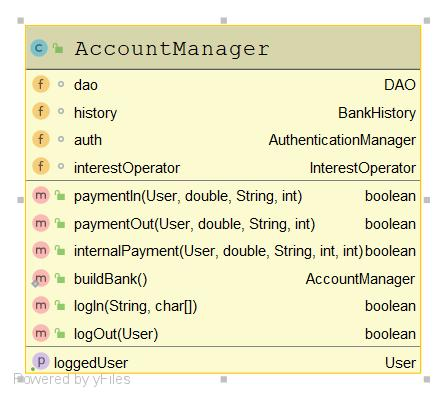
\includegraphics[width = 200pt]{DiagramKlasy.jpg}
\caption{Przykładowy diagram opisujący jedną klasę.}\label{diagram_wybranej_klasy}
\end{figure}

\begin{table}
\begin{tabularx}{\textwidth}{|l|X|}
\hline
&\textbf{Pobranie wybranego rekordu}\\\hline
URL &   \url{http://geniusgamedev.eu/cordova/rest_api/rest_srv/:id} lub \url{http://geniusgamedev.eu/cordova/rest_api/rest.php?id=:id}\\\hline
Method  & GET\\\hline
Parameters  & id - id wybranego elementu \\\hline
Request Data & None\\\hline
Response Data & obiekt w postaci:\\
&

%\begin{js}
\{'data':\{
    'id':2,
    'name':'Helena',
    'score':128
    \}
\}
%\end{js}

\\\hline
\end{tabularx}
\caption{Metoda get stosowanej usługi REST}\label{rest1}
\end{table}

\section{Cytowania}
Cytowania należy oznaczać wykorzystując {\textbackslash}cite. Wielokrotne cytowania należy grupować \cite{Bekart, Cytowanie, latex_math_wiki, Procedura_dyplomowania} W pracy należy stosować jeden z trzech systemów cytowań (Vancouver System, Harvard System, Oxford System) opisanych szczegółowo w \cite{Cytowanie}, regulamin dyplomowania zaleca wykorzystanie systemu \underline{Vancouver}. W~przypadku systemów Vancouver i Oxford bibliografia powinna być posortowana w kolejności pojawiania się odwołań w tekście, natomiast w systemie Harvard alfabetycznie wedle nazwisk pierwszych autorów.

\section{Spisy}
Praca musi zawierać spis treści {\textbackslash}tableofcontents oraz spis bibliograficzny, można również dodać spis rysunków  {\textbackslash}listoftables i spis tabel {\textbackslash}listoffigures. 

\listoftables
\listoffigures

\thebibliography{99}
\bibitem{Procedura_dyplomowania} Procedura dyplomowania na WFiIS UŁ:
\url{http://wfi.uni.lodz.pl/student/procedury-akty-prawne-i-formularze/#toggle-id-1}
\bibitem{latex_wiki} Wiki page about LaTeX: \url{https://en.wikibooks.org/wiki/LaTeX}.
\bibitem{Bekart} Strony Wikipedii poświęcone błędom w łamaniu tekstu\\
\url{https://pl.wikipedia.org/wiki/B%C4%99kart_(typografia)}
\bibitem{latex_math_wiki} Wiki page about LaTeX/Advanced Mathematics: \url{https://en.wikibooks.org/wiki/LaTeX/Advanced_Mathematics}.
\bibitem{Cytowanie} Strona Wikipedii poświęcona metodom cytowania \\
\url{https://pl.wikipedia.org/wiki/Cytowanie_pi%C5%9Bmiennictwa}


\bibitem{1}	A. De Vos, Reversible Computing: Fundamentals, Quantum Computing, and Applications. Weinheim: Wiley-VCH Verlag, Berlin (2010)
\bibitem{2}	M. Saeedi and I. L. Markov, ``Synthesis and Optimization of Reversible Circuits: A Survey,'' ACM Computing Surveys, vol. 45, no. 2, pp. 21:1-34, 2013
\bibitem{3}	M. Soeken, R. Wille, O. Keszocze, D. M. Miller, and R. Drechsler, ``Embedding of Large Boolean Functions for Reversible Logic,'' J. Emerg. Technol. Comput. Syst., vol. 12, no. 4, article 41, 26 pages, December 2015; also available as preprint arXiv.org:1408.3586, August 15, 2014
\bibitem{4}	C. Carlet, ``Vectorial Boolean Functions for Cryptography,'' in: Y. Crama and P. Hammer (Eds,), Boolean Models and Methods in Mathematics, Computer Science, and Engineering, pp. 398-472 Cambridge University Press, 2010
\bibitem{5}	N. Tokareva, Bent Functions. Results and Applications to Cryptography,'' Academic Press, London 2015
\bibitem{6}	P. Kerntopf, C. Moraga, K. Podlaski, and R. Stankovic, ``Towards Classification of Reversible Functions,'' In: Steinbach, B. (Ed.), Proceedings of the 12th International Workshop on Boolean Problems, September 2016, pp. 21-28
\bibitem{7}	P. Kerntopf, C. Moraga, K. Podlaski, and R. Stankovic, ``Towards Classification of Reversible Functions with Homogeneous Component Functions,'' In: Steinbach, B. (Ed.), Further Improvements in the Boolean Domain. Newcastle upon Tyne: Cambridge Scholars Publishing, 2018, pp. 386-406
\bibitem{8}	P. Kerntopf, K. Podlaski, C. Moraga, and R. Stankovic, ``Study of Reversible Ternary Functions with Homogeneous Component Functions,'' In: Proceedings of the 47th IEEE International Conference on Multiple-Valued Logic, May 2017, pp. 191-196
\bibitem{9}	P. Kerntopf, R. Stankovic, K. Podlaski, and C. Moraga, ``Ternary/MV Reversible Functions with Component Functions from Different Equivalence Classes,'' In: Proceedings of the 48th IEEE International Conference on Multiple-Valued Logic, May 2018, pp. 109-114
\bibitem{10}	P. Kerntopf, K. Podlaski, C. Moraga, and R. Stankovic, ``New Results on Reversible Boolean Functions Having Component Functions with Specified Properties,'' In: Soeken, M. (Ed.), Proceedings of the 13th International Workshop on Boolean Problems, September 2018, pp. 151-166
\bibitem{11}	C.-C. Tsai and M. Marek-Sadowska, ``Boolean Functions Classification via Fixed Polarity Reed-Muller Forms,'' IEEE Transactions on Computers, vol. 46, no. 2, pp. 173-186, February 1997
\bibitem{12}	D. Debnath and T. Sasao, ``Fast Boolean Matching under Variable Permutation Using Representative,'' Proceedings of the Asia and South Pacific Design Automation Conference, January 1999, pp. 359-362
\bibitem{13}	D. Debnath and T. Sasao, ``Efficient Computation of Canonical Form for Boolean Matching in Large Libraries,'' Proceedings of the Asia and South Pacific Design Automation Conference, January 2004, pp. 591-596
\bibitem{14}	D. Debnath and T. Sasao, ``Fast Boolean Matching under Permutation by Efficient Computation of Canonical Form,'' IEICE Transactions on Fundamentals of Electronics, vol. E87-A, December 2004, pp. 3134-3140
\bibitem{15}	D. Debnath and T. Sasao, ``Efficient Computation of Canonical Form under Variable Permutation and Negation for Boolean Matching in Large Libraries,'' IEICE Transactions on Fundamentals of Electronics, Communications and Computer Sciences, vol. E89-A, No.12, December 2006, Special Section on VLSI Design and CAD Algorithms, pp. 3443-3450
\bibitem{16}	R. S. Stanković, J. T. Astola, and B. Steinbach, ``Former and Recent Work in Classification of Switching Functions,'' in: Steinbach, B. (Ed.), Proceedings of the 8th International Workshop on Boolean Problems, September 2008, pp. 115-126
\bibitem{17}	C. S. Lorens, ``Invertible Boolean Functions,'' Space-General Corp., El Monte, CA, Re-search Memorandum No. 21; January 25, 1962 and July 1, 1962
\bibitem{18}	C. S. Lorens, ``Invertible Boolean Functions,'' IEEE Transactions on Electronic Computers, vol. EC-13, no. 5, pp. 529-541, October 1964
\bibitem{19}	M. A. Harrison, ``The Number of Classes of Invertible Boolean Functions,'' Journal of ACM, vol. 10, pp. 25-28, 1963
\bibitem{20}	I. E. Strazdins, ``On the Number of Types of Invertible Binary Networks,'' Avtomatika \& Vychislitelnaya Tekhnika, no. 1, pp. 30-34, 1974
\bibitem{21}	E. A. Primenko, ``Invertible Boolean Functions and Fundamental Groups of Transformations of Algebras of Boolean Functions,'' Avtomatika \& Vychislitelnaya Tekhnika, no. 3, pp. 17-21, 1976
\bibitem{22}	E. A. Primenko, ``On the Number of Types of Invertible Boolean Functions,'' Avtomatika \& Vychislitelnaya Tekhnika, no. 6, pp. 12-14, 1977
\bibitem{23}	E. A. Primenko, ``On the Number of Types of Invertible Transformations in Multivalued Logic,'' Kibernetika, no. 5, pp. 27-29, 1977
\bibitem{24}	E. A. Primenko, ``Equivalence Classes of Invertible Boolean Functions,'' Kibernetika, no. 6, pp. 1-5, 1984
\bibitem{25}	J. E. Rice, ``Considerations for Determining a~Classification Scheme for Reversible Boolean Functions,'' Technical Report TR-CSJR2-2007, University of Lethbridge, Department of Mathematics and Computer Science, Lethbridge, Alberta, Canada, 2007
\bibitem{26}	M. Soeken, N. Abdessaied, and G. De Micheli: ``Enumeration of Reversible Functions and Its Application to Circuit Complexity,'' In: S. Devitt, I. Lanese (Eds.), Reversible Computation. Proceedings of the 8th International Conference, RC 2016, Bologna, Italy, July 7–8, 2016, Lecture Notes in Computer Science, vol. 9720, pp. 255-270, Springer International Publishing AG Switzerland, 2016
\bibitem{27}	T. G. Draper, ``Nonlinear Complexity of Boolean Permutations'' Ph.D. thesis, University of Maryland, 2009
\bibitem{28}	S. Aaronson, D. Grier, and L. Schaeffer, ``The Classification of Reversible Bit Operations,'' Preprint arXiv:1504.05155 [quant-ph], 68 pages, April 20, 2015
\bibitem{29}	M. Caric and M. Zivkovic, ``On the Number of Equivalence Classes of Invertible Boolean Functions under Action of Permutation of Variables on Domain and Range,'' Publications de l'Institut Mathématique, vol. 100, no. 114, 2016, pp. 95–99, also available as preprint arXiv:1603.04386v2 [math.CO], 9 pages, April 6, 2016
%\bibitem{30}	R. E. Bryant, ``On the Complexity of VLSI Implementations and Graph Representations of Boolean Functions with Application to Integer Multiplication,'' IEEE Transactions on Computers, vol. 40, no. 2, pp. 205-213, 1991
%\bibitem{31}	B. Bollig, M. Löbbing, M. Sauerhoff, and I. Wegener, ``On the Complexity of the Hidden Weighted Bit Function for Various BDD Models,'' Informatique Theorique et Applications, vol. 33, pp. 103-116, 1999
%\bibitem{32}	D. Maslov, Personal communication, July 2016
\bibitem{33}	J. Jegier, P. Kerntopf, and M. Szyprowski, ``An Approach to Constructing Reversible Multi-Qubit Benchmarks with Provably Minimal Implementations,'' In: Proceedings of the 13th IEEE International Conference on Nanotechnology, pp. 99-104, 2013
\bibitem{34}	J. Jegier, P. Kerntopf, ``Progress Towards Constructing Sequences of Benchmarks for Quantum Boolean Circuits Synthesis,'' In: Proceedings of the 14th IEEE International Conference on Nanotechnology, pp. 250-255, 2014

\end{document}
